\section{Auswertung}
\label{sec:Auswertung}
In der folgenden Tabelle sind alle Messwerte aufgeführt
\begin{table}
  \centering
  \caption{Messdatentabelle.}
  \label{tab:Data}
  \begin{tabular}{c c c c c c}
    \toprule
    $Zeit/s$ & $T_1/K$ & $T_2/$ & $p_a/\text{bar}$ & $p_b/\text{bar}$ & $N/W$ \\
    \midrule
    0  &  21.7  &  21.9  &  4.1  &   4.2  &  170 \\
    1  &  22.1  &  21.8  &  1.4  &   6.0  &  170 \\
    2  &  23.3  &  21.8  &  1.8  &   6.2  &  180 \\
    3  &  24.6  &  20.9  &  2.0  &   6.7  &  190 \\
    4  &  26.2  &  19.4  &  2.1  &   7.2  &  195 \\
    5  &  28.0  &  17.6  &  2.1  &   7.3  &  200 \\
    6  &  29.9  &  15.8  &  2.1  &   8.0  &  200 \\
    7  &  32.0  &  14.1  &  2.1  &   9.0  &  205 \\
    8  &  35.1  &  12.3  &  2.1  &   9.5  &  205 \\
    9  &  37.5  &  10.7  &  2.1  &   9.9  &  208 \\
   10  &  36.9  &   9.0  &  2.1  &   9.4  &  210 \\
   11  &  38.8  &   7.4  &  2.1  &  10.7  &  208 \\
   12  &  40.4  &   6.0  &  2.1  &  10.0  &  208 \\
   13  &  42.1  &   4.4  &  2.1  &  10.4  &  210 \\
   14  &  43.6  &   3.0  &  2.1  &  10.9  &  210 \\
   15  &  45.2  &   1.6  &  2.2  &  11.0  &  210 \\
   16  &  46.7  &   0.5  &  2.2  &  11.5  &  210 \\
   17  &  48.0  &  -0.3  &  2.2  &  12.0  &  210 \\
   18  &  49.5  &  -0.7  &  2.2  &  12.1  &  210 \\
   19  &  50.7  &  -1.0  &  2.2  &  12.5  &  210 \\
   \bottomrule
 \end{tabular}
\end{tabel}

Die Temperaturverläufe sind in dem folgenden Diagramm dargestellt und mit einer
linearen Ausgleichstrechnung approximiert.
\subsection{Aufgabe. a}
\begin{figure}
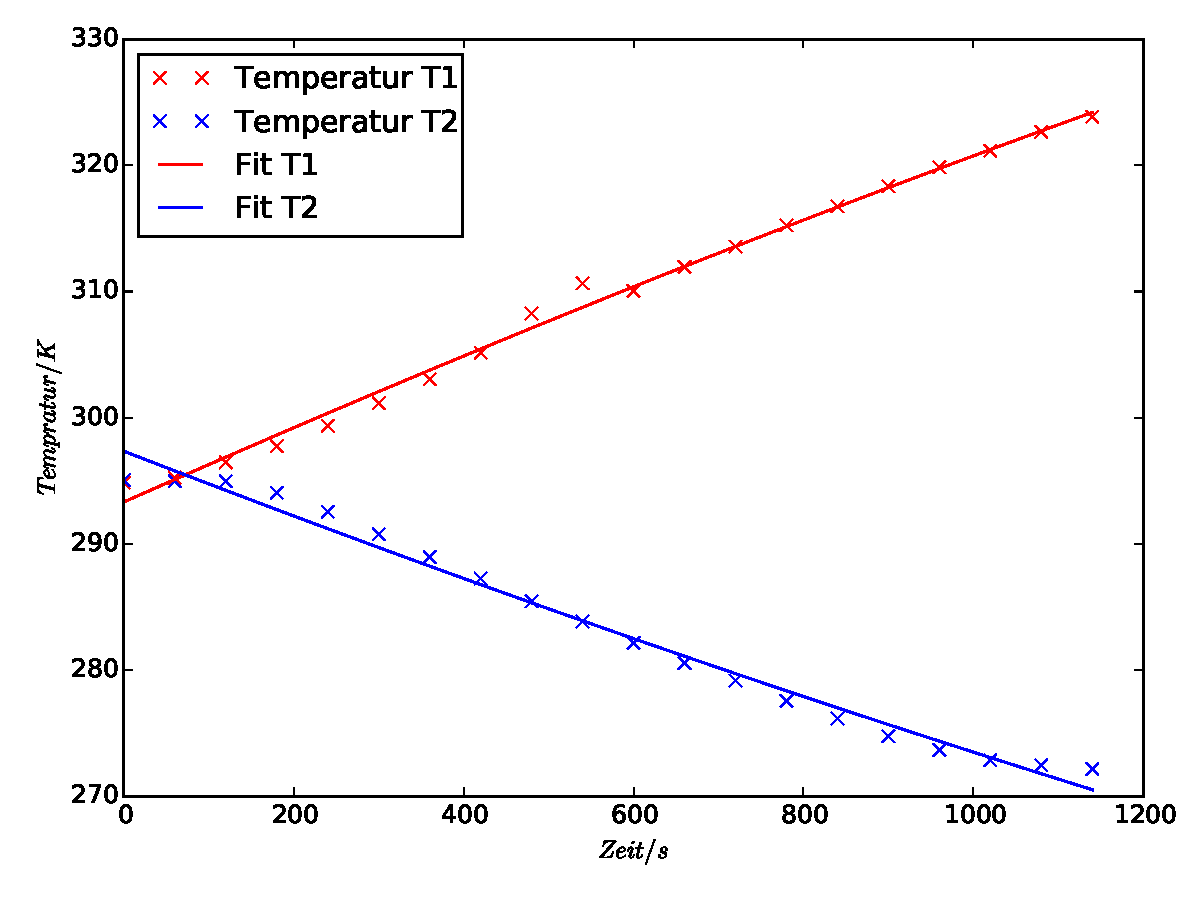
\includegraphics[height=13cm]{Temperaturgraphik.pdf}
\end{figure}
%\usepackage{pdfpages}
%  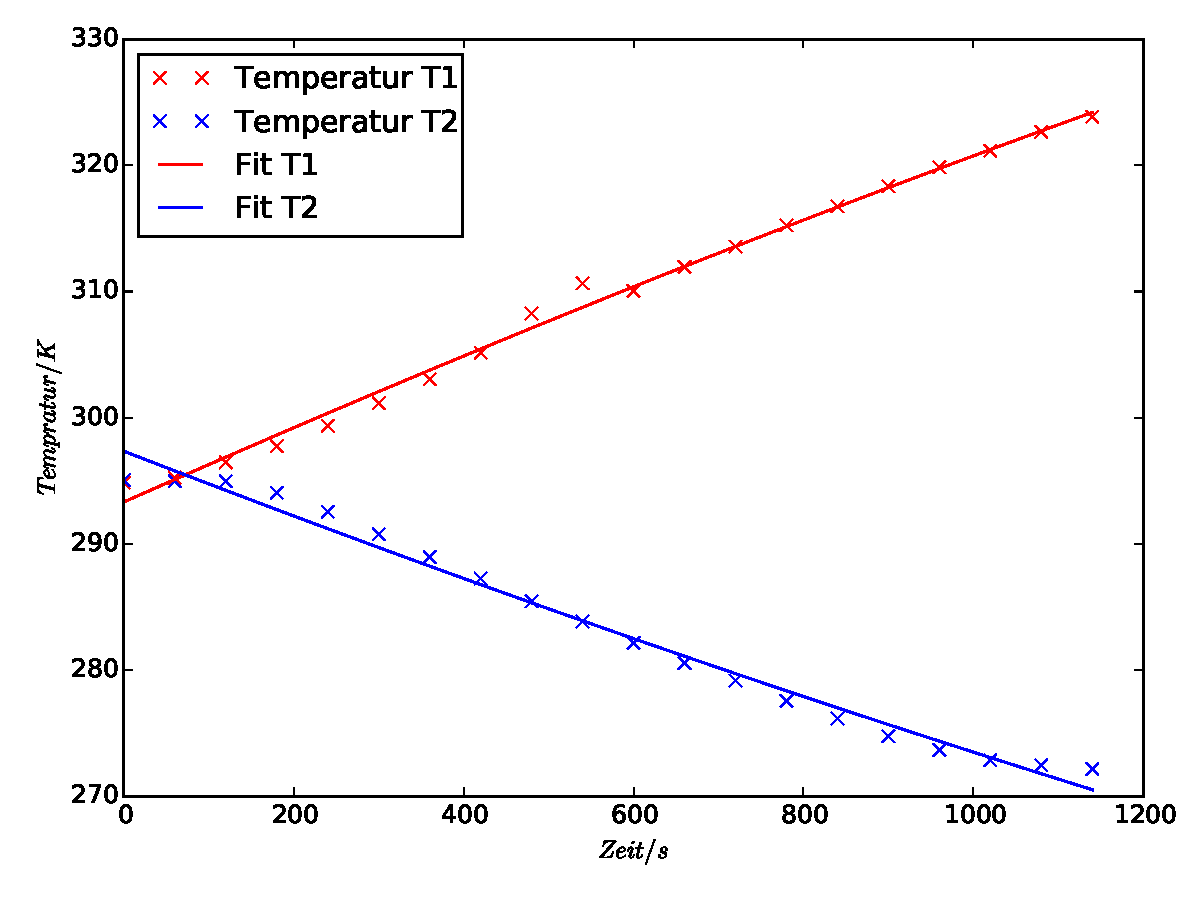
\includepdf[pages=-]{Temperaturgraphik.pdf}
Die Näherung wurde mit scientific Python gemacht und ist gegeben durch
\begin{equation}
  T(t)=At^2+Bt+C .
\end{equation}
Die Parameter für erwärmte Reservoir $T_1$ sind
\begin{equation}
  A=(  -0.000002485)\frac{K}{s^2}
  B=(   0.029925168)\frac{K}{s}
  C=( 293.312793014)K
\end{equation}
Die Parameter für den anderen Behälter$T_2$ sind
\begin{equation}
  A=(  0.000002259)\frac{K}{s^2}
  B=( -0.026112097)\frac{K}{s}
  C=(297.339350549)K

\end{equation}
Die dazugehörigen Differentialquotienten erhält man durch die folgende Gleichung
\begin{equation}
\frac{dT}{dt}=At^2+B
\end{equation}

\begin{table}
  \centering
  \caption{Differentialquotienten.}
  \label{tab:Diffquo}
  \begin{tabular}{c c c}
    \toprule
    $Zeit/s$ & $dT_1 /dt$ & $dT_2 /dt$ \\
    \midrule
    300  &  0.02843375268378217635 & -0.02475643627514830664  \\
    600  &  0.02694233722154850894 & -0.02340077471351255378  \\
    900  &  0.02545092175931483805 & -0.02204511315187679746  \\
   1140  &  0.02425778938952790134 & -0.02096058390256819171  \\
   \bottomrule
 \end{tabular}
\end{tabel}
Als nächstes soll die Güteziffer bestimmt werden dafür Nutzt man die Gleichung
\eqref{eqn:gueteziffer_ideal} für die ideale Güteziffer und die Gleichung
\eqref{eqn:gueteziffer_real}
\begin{table}
  \centering
  \caption{Güteziffer}
  \label{tab:Gütez}
  \begin{tabular}{c c c}
    \toprule
    $Zeit/s$ & $v_id$ &  $v_re$ \\
    \midrule
      300  &  28.95673076923083045  &  1.874590179809934698 \\
      600  &  11.11290322580645906  &  1.691679648289791338 \\
      900  &  7.301605504587160844  &  1.598035315808215895 \\
     1140  &  6.264023210831721755  &  1.523119849822955674 \\
   \bottomrule
 \end{tabular}
\end{tabel}
Wenn man die Werte in Gleichung \eqrref{eqn:massendurchsatz} einsetzt erhält man
den Massendurchsatz.
\begin{tabel}
  \centering
  \caption{Massendurchsatz}
  \label{tab:Massend}
\begin{tabular}{c c}
  \toprule
  $Zeit /s$ & $dQ_2 /dt$ & $dm/dt (mol/s)$  \\
  \midrule
  300  &   -326.4301609752228615  & -0.01394630925991996971  \\
  600  &   -308.5548570795280057  & -0.01318260986553914521  \\
  900  &   -290.6795531838330362  & -0.01241891047115831551  \\
 1140  &   -276.3793100672771175  & -0.01180795095565365452  \\
 \bottomrule
\end{tabular}
\end{tabel}

Die Dichte \roh ,die für die Berechnung mechanischen Kompressorleistung
benötigt wird, kann berechnet werden, indem man die Gleichung der idealen Gase
umstellt.
\begin{equation}
  pV=nRT \leftrightarrow \frac{pV}{T}=nR
\end{equation}
Damit ergibt sich, da die Stoffmenge $n$ konstant bleibt,
\begin{equation}
  n_1=n_2
  \frac{p_0 V_0}{T_0}=\frac{p_2 V_2}{T_2}
\end{equation}
Da $ \roh V=m$ \leftrightarrow $V= \frac{m}{\roh}$ lässt sich \roh bestimmen wobei
$\roh_2=\roh$ und $p_2=p_a$.
\begin{equation}
  \roh=\frac{\roh_0 T_0 p_a}{T_2 p_0}
\end{equation}
Und mit Gleichung \eqref{eqn:kompressorleistung}
\begin{equation}
N_mech=\frac{1}{\kappa-1}\left(p_b \sqrt[\kappa]{\frac{p_a}{p_b}}-p_a\right)\frac{1}{\frac{\roh_0 T_0 p_a}{T_2 p_0}}\frac{dm}{dt}
\end{equation}
